% Created 2018-11-26 月 15:51
% Intended LaTeX compiler: pdflatex
\documentclass[presentation,dvipdfmx,CJKbookmarks]{beamer}
\usepackage{CJKutf8}
\usepackage{atbegshi}
\AtBeginShipoutFirst{\special{pdf:tounicode UTF8-UTF16}} % for UTF-8
\usepackage[utf8]{inputenc}
\usepackage[T1]{fontenc}
\usepackage{graphicx}
\usepackage[export]{adjustbox}
\usepackage{lmodern}
\usepackage{grffile}
\usepackage{longtable}
\usepackage{wrapfig}
\usepackage{rotating}
\usepackage[normalem]{ulem}
\usepackage{amsmath}
\usepackage{textcomp}
\usepackage{amssymb}
\usepackage{capt-of}
\usepackage{hyperref}
 \usepackage{minted}
\usetheme{Boadilla} \usecolortheme{crane}
\usecolortheme{lily}
\author{Bao Haojun}
\date{2015-11-20}
\title{System-config: Wishful Thinking}
\hypersetup{
 pdfauthor={Bao Haojun},
 pdftitle={System-config: Wishful Thinking},
 pdfkeywords={},
 pdfsubject={},
 pdfcreator={Emacs 26.1 (Org mode 9.1.9)}, 
 pdflang={English}}
\begin{document}
\begin{CJK*}{UTF8}{simsun}

\maketitle
\begin{frame}{Outline}
\tableofcontents
\end{frame}

\CJKtilde

\section{Wishful Thinking}
\label{sec:org1a70d08}

\section{一种有意思的UX:交互式补齐}
\label{sec:org1f3c5e4}
\begin{frame}[label={sec:org2ffb0b5}]{在Firefox中}
\begin{center}
\includegraphics[width=.9\linewidth]{./images/firefox.ps}
\end{center}
\end{frame}

\begin{frame}[label={sec:orgcd7abf9}]{在Emacs中}
\begin{center}
\includegraphics[width=.9\linewidth]{./images/emacs.ps}
\end{center}
\end{frame}

\begin{frame}[label={sec:org7f9bd72}]{在文件管理器中?}
\begin{center}
\includegraphics[width=.9\linewidth]{./images/file-manager.ps}
\end{center}
\end{frame}

\begin{frame}[label={sec:orgcac917b}]{在命令行上}
\begin{center}
\includegraphics[width=.9\linewidth]{./images/ui-cli.ps}
\end{center}
\end{frame}

\begin{frame}[label={sec:org0658029}]{在命令行上(2)}
\begin{block}{s (search engine)}
\end{block}
\begin{block}{git checkout -B}
\end{block}
\begin{block}{git cherry-pick}
\end{block}
\end{frame}


\begin{frame}[label={sec:orgdc9eddf}]{在小扳手里}
\begin{center}
\includegraphics[width=.9\linewidth]{./images/wrench-ui.ps}
\end{center}
\end{frame}

\begin{frame}[label={sec:org9e5adc6}]{到处都是}
\begin{block}{窗口管理器}
\end{block}
\begin{block}{Emacs的几乎所有命令——helm}
\end{block}
\begin{block}{命令行上的变种}
\end{block}
\begin{block}{在输入法里}
\end{block}
\begin{block}{在Smartisan手机里,邮件联系人搜索}
\end{block}
\end{frame}

\section{最重要的7种武器}
\label{sec:org93cb08a}
\begin{frame}[label={sec:org0955fb3}]{编辑器(Emacs)}
\begin{block}{一切皆文本,不管是程序,还是文档}
\end{block}
\begin{block}{各种更强大的补齐}
\begin{itemize}
\item C/C++语言 (Qt/Visual C++)
\item Java
\item bbyac
\item yasnippet
\item codegen
\item getopts/getopt
\end{itemize}
\end{block}
\begin{block}{利用Emacs阅读源代码}
\end{block}
\end{frame}

\begin{frame}[label={sec:org3bd59af}]{Emacs续(阅读源代码)}
\begin{block}{beagrep}
\end{block}
\begin{block}{grep-beatags}
\end{block}
\begin{block}{grep-func-call}
\end{block}
\begin{block}{查local变量的定义}
\end{block}
\begin{block}{查local变量的使用}
\end{block}
\end{frame}
\begin{frame}[label={sec:orgd9ae5c1}]{Emacs续(查文档)}
\begin{block}{man手册}
\end{block}
\begin{block}{info}
\end{block}
\begin{block}{html——交给firefox}
\end{block}
\end{frame}
\begin{frame}[label={sec:orgce9438c}]{命令行(xfce4-terminal + bash)}
\begin{block}{历史机制}
\begin{itemize}
\item bash自带
\item re
\item cd的历史机制
\end{itemize}
\end{block}
\begin{block}{各种工具的无限组合}
\begin{itemize}
\item of
\item putclip
\item 切下当前命令行输入的快捷键
\item up/swp
\end{itemize}
\end{block}
\end{frame}
\begin{frame}[label={sec:orgaebad94}]{浏览器(firefox)}
\begin{block}{像Emacs一样的按键(看萨苏的博客)}
\end{block}
\begin{block}{可以自己写monkeygrease脚本}
\end{block}
\begin{block}{可以当我的文档工具}
\end{block}
\begin{block}{可以当我的字典}
\end{block}
\end{frame}
\begin{frame}[label={sec:org38b65d9}]{桌面管理器(sawfish)}
\begin{block}{为其他所有工具的集成提供辅助}
\begin{itemize}
\item 为Emacs阅读代码提供辅助
\item 为Qt Creator与Emacs切换提供辅助
\end{itemize}
\end{block}
\begin{block}{自定义快捷键}
\end{block}
\begin{block}{像Vim那样,可以有模式的概念}
\end{block}
\begin{block}{让所有程序的文字输入,都支持基本的Emacs快捷键}
\end{block}
\end{frame}

\begin{frame}[label={sec:orge17fc2d}]{版本管理工具}
\begin{block}{Git与Emacs、脚本的集成 refactory-rename}
\end{block}
\begin{block}{ew uu}
\end{block}
\begin{block}{git-interactive-add}
\end{block}
\begin{block}{没有版本管理工具,就没有system-config}
\end{block}
\begin{block}{开始任何项目,先创建 git 库!!!}
\end{block}
\end{frame}

\begin{frame}[label={sec:orge7d8d63}]{Linux}
\begin{block}{为什么这些工具如此重要?}
\begin{itemize}
\item 允许用户沉浸在里头
\item 我不讨厌鼠标,但讨厌切换
\begin{itemize}
\item 为什么要做字典的鼠标选词、查询功能
\end{itemize}
\end{itemize}
\end{block}
\end{frame}

\begin{frame}[label={sec:orgeddfc5f}]{自己}
\begin{block}{再好的工具,还是要靠人来用}
\end{block}
\end{frame}
\section{总结}
\label{sec:org747c2c6}
\begin{frame}[label={sec:org7672c40}]{s: 名字为什么这么短}
\begin{block}{海明码原理和优化}
\end{block}
\begin{block}{容易的事情更容易}
\end{block}
\begin{block}{难的事情变容易}
\end{block}
\begin{block}{不可能的事情变可能}
\end{block}
\begin{block}{分N步的事情变1步}
\end{block}
\begin{block}{大项目分解成小项目}
\end{block}
\begin{block}{自顶向下与自下而上}
\end{block}
\end{frame}
\begin{frame}[label={sec:org5332b22}]{许愿式编程}
\begin{block}{jwz的编程方法}
\begin{itemize}
\item org-mode介绍
\item GTD
\end{itemize}
\end{block}
\begin{block}{Linus的编程方法}
\end{block}
\begin{block}{sicp 和 htdp}
\end{block}
\end{frame}
\begin{frame}[label={sec:org4dded1d}]{高效编辑器的七种习惯}
\begin{block}{不要试图一下子学太多,够用就好}
\end{block}
\begin{block}{快来fork我的system-config项目吧}
\begin{itemize}
\item \url{https://github.com/baohaojun/system-config}
\end{itemize}
\end{block}
\begin{block}{快开始学Emacs吧}
\end{block}
\end{frame}

\begin{frame}[label={sec:org9c40df9}]{致谢}
\begin{block}{王垠}
\end{block}
\begin{block}{锤子科技、老板、同事}
\end{block}
\end{frame}
\end{CJK*}
\end{document}
